





\chapter{基于蒸馏的快速采样方法}\label{ch:distillation}

本章讨论如何用训练来加速采样。\emph{蒸馏}让学生生成器向采样较慢的预训练扩散模型学习。教师模型可能需要数百步，学生模型用几步就可以达到相近的质量\footnote{这里所说的蒸馏，压缩的是采样步数。}。上一章通过改进数值求解器来加速积分，本章则直接训练生成器。两种主要方法分别是\emph{分布层面的蒸馏}与\emph{流映射层面的蒸馏}。前者让学生模型匹配教师模型的输出分布，可以省去完整的轨迹模拟。后者训练学生用更少的步数重现教师的采样轨迹。



\chapterlearning{

  \item 区分两个主要的蒸馏目标：教师的分布及其状态到状态的流映射；

  \item 了解分布级蒸馏，学生通过基于分数的监督来匹配教师模型的噪声边缘；

  \item 了解流映射蒸馏，其中学生学习教师生成的转换，渐进式蒸馏逐步用一个学生步骤取代两个教师步骤。

}{以预先训练的扩散模型作为教师，本章的关键区别是学生被训练重现的内容：教师的分布或其流映射。下一章将探讨如何在没有教师模型的情况下学习如此快速的映射。}







\clearpage
\newpage


\section{序言}\label{sec:distillation-prologue}
扩散模型的一个核心瓶颈是采样太慢。由 Tweedie 公式（\Cref{subsec:four-equiv-para}）可知，扩散模型可以看成一种「$\rvx$-预测」模型：训练好的 $\rvx_{\bm{\phi}^\times}(\rvx_t, t)$ 能够从噪声输入 $\rvx_t$ 中还原出在噪声水平 $t$ 下的期望干净数据，
\[
    \rvx_{\bm{\phi}^\times}(\rvx_t, t) \approx \mathbb{E}[\rvx_0 |\rvx_t],
\]
其中期望取自 $p(\rvx_0 |\rvx_t)$，即与 $\rvx_t$ 相符的所有可能的干净数据。一个自然的想法是直接用 $\rvx_{\bm{\phi}^\times}(\rvx_t, t)$ 一步生成。然而这种去噪器要对许多看似合理的结果取平均，预测往往会过于平滑，只用少数几步去噪便只能得到模糊、低质的样本。

另一方面，正如 \Cref{subsec:sde-sample} 所讨论的，扩散采样是通过一长串迭代步骤沿 ODE 或 SDE 轨迹推进的。这能产生高保真的样本，但反复调用神经网络使采样代价高昂。对 $n$ 阶确定性 ODE 求解器，在标准正则性假设下，局部截断误差为 $\mathcal{O}(h^{n+1})$，固定时间区间上的全局离散化误差为 $\mathcal{O}(h^n)$，其中 $h=\max_i |t_i-t_{i-1}|$ 为步长。因此，用更粗的离散化通常会增大在一个固定学得向量场上引入的数值误差，尽管样本保真度并不一定随求解步数单调变差。于是，采样精度与计算成本之间就出现了实际的权衡。为突破这一瓶颈，一条主要的研究路线是\emph{蒸馏}：在能访问训练好的扩散模型（\emph{教师}）的前提下，训练一个生成器（\emph{学生}），使其用一次前馈或少数几步计算就重现教师的行为。这就把教师的许多采样步压缩成一个快速过程，从而绕开缓慢的迭代求解器，同时保持较高的样本保真度。下面介绍蒸馏的两种视角：\emph{分布层面的蒸馏}与\emph{流映射层面的蒸馏}\footnote{从时间顺序看，流映射层面的蒸馏出现更早：\emph{知识蒸馏}（KD）~\citep{luhman2021knowledge} 发表于 2021 年，\emph{渐进式蒸馏}（PD）~\citep{salimans2021progressive} 发表于 2022 年，都早于 2023 年前后成型的分布层面蒸馏方法族。不过为叙述顺畅、便于衔接下一章，我们先介绍分布层面的蒸馏。}。





\subsection{分布层面的蒸馏}  
分布层面的蒸馏旨在训练一个一步生成器 $\rmG_{\bm{\theta}}(\rvz)$，
把噪声 $\rvz \sim p_{\mathrm{prior}}$ 映射为样本
$\hat\rvx = \rmG_{\bm{\theta}}(\rvz)$，使其诱导分布
$p_{\bm{\theta}}(\hat\rvx)$ 逼近目标数据分布 $p_{\mathrm{data}}(\rvx)$。
这通常通过最小化某种统计差异来实现：
\[
\min_{\bm{\theta}}  \mathcal{D}\!\left(p_{\bm{\theta}}(\hat\rvx),  p_{\mathrm{data}}(\hat\rvx)\right),
\]
其中 $\mathcal{D}$ 表示合适的散度，例如 KL 散度。实际做法中，
基于分布的方法让生成器的分布去对齐预训练扩散模型所诱导的
经验分布 $p_{\bm{\phi}^\times}(\rvx)$：
\[
\min_{\bm{\theta}}  \mathcal{D}\!\left(p_{\bm{\theta}}(\hat\rvx),  p_{\bm{\phi}^\times}(\hat\rvx)\right),
\]
即用 $p_{\bm{\phi}^\times}$ 代替 $p_{\mathrm{data}}$。这类方法并不显式地
计算该散度，而是借助预训练的教师模型，以及按学生当前分布估计出的量，
为它的梯度构造一个可计算的估计式。在基于 KL 的分布匹配下，
这一梯度就表现为学生分数函数与目标分数函数之差。

这一形式通过分布对齐把扩散模型的多步生成过程蒸馏成单步模型。
我们在 \Cref{sec:VSD} 中详细介绍这类方法。




\subsection{流映射层面的蒸馏} 考虑 PF-ODE，它可以写成任意一种预测模型的形式（参见 \Cref{eq:predictions-equivalence}）：
\begin{align}\label{eq:pf-ode-ct}
    \frac{\diff \rvx(\tau)}{\diff \tau} 
    = f(\tau) \rvx(\tau) - \tfrac{1}{2}g^2(\tau) \nabla_\rvx \log p_\tau(\rvx(\tau)) 
    =: \rvv^*(\rvx(\tau), \tau).
\end{align}

其解映射（流映射）把时刻 $s$ 的状态 $\rvx_s$ 沿反向时间演化到
$t \leq s$，记作 $\bPsi_{s\to t}(\rvx_s)$，即
\begin{align}\label{eq:int_target_gt}
\begin{aligned}
    \bPsi_{s\to t}(\rvx_s) 
    &\coloneqq \rvx_s + \int_s^t \rvv^*(\rvx(\tau), \tau) \diff \tau,
\end{aligned}
\end{align}
其中积分即求解 PF-ODE。直观地说，$\bPsi_{s\to t}$ 把时刻 $s$ 的噪声状态
$\rvx_s$ 输运到噪声更小的时刻 $t$（最终数据位于 $t=0$）。
从扩散模型采样，就相当于对 $\rvx_T \sim p_{\mathrm{prior}}$ 求
$\bPsi_{T\to 0}(\rvx_T)$。通常这一积分要借助速度场 $\rvv$ 的迭代数值求解器
来近似（参见 \Cref{ch:solvers}），而这需要很多步（例如即便用
DPM-Solver 也要至少 $10$–$20$ 次 NFE），于是采样速度就比 GAN 这类
经典的一步生成模型慢。这就自然引出下面的问题：
\begin{question}
    能否直接学习解映射 $\bPsi_{s\to t}(\rvx_s)$？
\end{question}
特别地，若能学到 $\rvx_T \sim p_{\mathrm{prior}}$ 下的映射
$\bPsi_{T\to 0}(\rvx_T)$，就实现了一步生成。


\paragraph{轨迹蒸馏。}

轨迹蒸馏的目标是训练一个神经网络生成器，使其在单个样本的层面上
近似解映射。由于 PF-ODE 的积分很少能写成闭式，训练时必须对它作
数值近似。为便于表述，引入通用的求解器记号
\begin{align}\label{eq:solver}
    \mathtt{Solver}_{s\to t}(\rvx_s;\,\bm{\phi}^\times)
    \quad \text{or simply} \quad
    \mathtt{Solver}_{s\to t}(\rvx_s),
\end{align}
它表示以 $\rvx_s$ 为初值、从 $s$ 积分到 $t$ 的经验 PF-ODE 的
数值解，其中教师参数为 $\bm{\phi}^\times$（上下文清楚时从略）。



\paragraph{早期方法：直接知识蒸馏。}
为实现少步乃至一步生成，一种直接的做法是训练生成器
$\rmG_\btheta(\rvx_T, T,0)$，让它模仿沿完整轨迹求值的数值求解器的输出：
\[
\rmG_\btheta(\rvx_T, T,0)\approx \mathtt{Solver}_{T\to 0}(\rvx_T), 
\qquad \rvx_T \sim p_{\mathrm{prior}}.
\]
这一想法正是最早的轨迹蒸馏方法之一\emph{知识蒸馏}
~\citep{luhman2021knowledge} 的基础，其回归损失为
\[
\mathcal{L}_{\mathrm{KD}}(\btheta)
:= 
\E_{\rvx_T \sim p_{\mathrm{prior}}}
\left\|
\rmG_\btheta(\rvx_T, T,0)
-
\mathtt{Solver}_{T\to 0}(\rvx_T)
\right\|_2^2.
\]
这种方法虽然能直接利用预训练教师提供的监督，却用不上原始训练数据中
那份更强的监督。此外，若在训练循环里调用 ODE 积分，计算代价会很高，
因为每次参数更新都要先解一遍 ODE 才能得到回归目标。最后，
由于生成器只学了一个从 $T$ 到 $0$ 的全局映射，它可能丧失
从中间状态引导生成过程的可控性；因此 \Cref{ch:guidance} 中介绍的
多数可控生成技术无法直接套用。




\paragraph{渐进式蒸馏概述。}
\emph{渐进式蒸馏}（PD）~\citep{salimans2021progressive} 借助教师的
\emph{局部}片段来训练一个带时间条件的 $\mathtt{Student}$。
设 $t_0=T>t_1>\cdots>t_N=0$ 为固定时间网格，教师提供
各段时间步进映射 $\mathtt{Teacher}_{t_k\to t_{k+1}}$，
$k=0,\ldots,N-1$。PD 并不只监督 $T\to 0$ 这一大步，
而是让 $\mathtt{Student}$ 去匹配教师连续两步所对应的两步跳跃映射：
\[
\mathtt{Student}_{t_k\to t_{k+2}}
\;\approx\;
\mathtt{Teacher}_{t_{k+1}\to t_{k+2}}
\circ
\mathtt{Teacher}_{t_{k}\to t_{k+1}},
\]
其中 $k = 0, 2, 4, \dots$。匹配用一个简单的回归损失（例如均方误差）来实现。
在这些局部配对片段上训练完毕之后，$\mathtt{Student}$ 就不再走原网格的
每一个时间间隔，而是每隔一个时间点前进一步，
\[
t_0 \to t_2 \to t_4 \to \cdots \to t_N,
\]
这意味着 $\mathtt{Student}$ 的每一步实际上覆盖了
$\mathtt{Teacher}$ 连续的两步。于是 $\mathtt{Student}$ 只用
$N/2$ 次转移就覆盖了同样的总时间跨度 $[0,T]$。这一阶段结束后，
训练好的 $\mathtt{Student}$ 取代 $\mathtt{Teacher}$ 成为新的参考模型。
随后在更粗的网格上重复整个过程，时间点数每次减半
（$N \to N/2 \to N/4 \to \cdots$），把轨迹逐步压缩成越来越少的步骤，
直到达到所需的推理步数。这种反复对半的做法在保持全局时间跨度的同时，
不断降低生成过程的时间分辨率。






\paragraph{流映射学习的统一视角。}
包括 KD 与 PD 在内的各类方法，都可以纳入同一个损失框架：
\begin{align}\label{eq:general-cm-loss}
  \mathcal{L}_{\mathrm{oracle}}(\btheta)
  := \E_{s,t} \E_{\rvx_s \sim p_s} 
  \left[  w(s,t)  d \big(\rmG_\btheta(\rvx_s, s,t),  \bPsi_{s\to t}(\rvx_s)\big)\right],
\end{align}
其中 $\bPsi_{s\to t}$ 是预言量形式的流映射，$w(s,t) \geq 0$ 指定
各时间对 $(s,t)$ 的加权方式，$d(\cdot,\cdot)$ 是某种差异度量，例如
$d(\rvx,\rvy)=\|\rvx-\rvy\|_2^2$ 或 $d(\rvx,\rvy)=\|\rvx-\rvy\|_1$，
$p_s$ 表示时刻 $s$ 的前向噪声边缘。由于 $\bPsi_{s\to t}$ 没有闭式，
只能依靠近似值，通常来自预训练的扩散模型（教师）或其他便于计算的替身。
KD 只是 \Cref{eq:general-cm-loss} 的一个简单特例：只取端点对
$(s,t)=(T,0)$。等价地，也可取退化的权重
$w(s,t)=\delta(s{-}T)\delta(t)$。若设 $p_T=p_{\mathrm{prior}}$
\footnote{当噪声调度恰好在 $T$ 处到达先验时该等式成立；
否则通常取足够大的 $T$ 使 $p_T\approx p_{\mathrm{prior}}$。}，
则预言量目标变为
\[
\E_{\rvx_T\sim p_T}
\big\|\rmG_\btheta(\rvx_T,T,0)-\bPsi_{T\to 0}(\rvx_T)\big\|_2^2
\approx \mathcal{L}_{\mathrm{KD}}(\btheta),
\]
而实用的 KD 目标则把预言量流映射换成
$\mathtt{Solver}_{T\to 0}\approx\bPsi_{T\to 0}$。关于这一表述的另一种
看法见 \Cref{app-sec:flow-map}。PD 同样能纳入这一模板：它不只用
单个端点对 $(T,0)$ 作监督，而是取许多\emph{相邻}时间对，
并施加一条简单的\emph{局部一致性}要求——先走一小步再走一小步，
应当与一步直接跨越两步的结果相符。我们在 \Cref{eq:pd-local}
处再回到这一点。

实践中最大的困难在于预言量流映射 $\bPsi_{s\to t}$ 一般没有闭式表达，
因此无法直接用作监督。为有效地逼近这一目标，已经发展出一系列方法，
但它们的成功往往取决于教师模型的质量。我们会在
\Cref{ch:fast-scratch} 中回到 \Cref{eq:general-cm-loss}，
给出一个从头训练方法的原则性框架，把教师排除在学习循环之外。








\clearpage
\newpage



\section{\texorpdfstring{基于分布的蒸馏}{基于分布的蒸馏}}\label{sec:VSD}


有多项工作以不同名称追求这类分布层面的蒸馏，包括分布匹配蒸馏（DMD）
~\citep{yin2024one,yin2024improved}、变分分数蒸馏（VSD）
~\citep{pooledreamfusion,wang2023prolificdreamer,luo2023diff,lu2024simplifying}
以及分数恒等蒸馏（SiD）~\citep{zhou2024score}。它们在技术细节上虽有差异，
遵循的原则却是同一个：训练一个生成器，使其前向噪声边缘与教师的边缘相匹配。
下面以 VSD 作为代表性表述来展开，因为其余做法也遵循类似的原则。\footnote{
从历史上看，VSD~\citep{wang2023prolificdreamer} 是为文本到 3D 生成引入的，
其中预训练的 2D 扩散模型通过可微渲染器提供分布监督。它取单粒子
（狄拉克）特例时，便退化为基本的 SDS~\citep{pooledreamfusion} 更新，
只相差相应的时间加权与预测参数化约定。
}


\subsection{以 VSD 为例}
\paragraph{前向过程。}
设 $\{p_t\}_{t \in [0,T]}$ 表示下述前向扩散过程的边缘密度
\[
\rvx_t = \alpha_t \rvx_0 + \sigma_t \bm{\epsilon}, \quad \bm{\epsilon} \sim \mathcal{N}(\bm{0}, \rmI),
\]
其初始分布为 $p_0 = p_{\mathrm{data}}$。另记 $p_0^{\bm{\theta}}$ 为
确定性一步生成器 $\rmG_{\bm{\theta}}(\rvz)$ 在隐变量
$\rvz \sim p_{\mathrm{prior}}(\rvz)$ 下所产生的合成样本分布。
再把 $\{p_t^{\bm{\theta}}\}_{t \in [0,T]}$ 定义为对 $p_0^{\bm{\theta}}$
施加同一前向扩散过程所得的边缘密度，即
\begin{align}\label{eq:vsd-forward}
    \rvx_t^{\bm{\theta}} := \alpha_t \rmG_{\bm{\theta}}(\rvz) + \sigma_t \bm{\epsilon}, 
\end{align}
其中 $\rvz \sim p_{\mathrm{prior}}$，$\bm{\epsilon} \sim \mathcal{N}(\bm{0}, \rmI)$。
可见 $p_t$ 与 $p_t^{\bm{\theta}}$ 共用同一个高斯扩散核
$p_t(\rvx_t| \rvx_0)$，区别只在于起始分布不同
（分别为 $p_{\mathrm{data}}$ 与一步合成样本分布 $p_0^{\bm{\theta}}$）。

\paragraph{训练目标和梯度。}
文献中通常用 KL 散度来匹配 $p_t$ 与 $p_t^{\bm{\theta}}$，
即最小化
\begin{align*}
    \mathcal{L}_{\text{VSD}}(\bm{\theta}) :=\mathbb{E}_t \left[ \omega(t)  \mathcal{D}_{\text{KL}}(p_t^{\bm{\theta}} \, \| \, p_t) \right]
= \mathbb{E}_{t, \rvz, \bm{\epsilon}} \left[ \omega(t) \left( \log p_t^{\bm{\theta}}(\rvx_t^{\bm{\theta}}) - \log p_t(\rvx_t^{\bm{\theta}}) \right) \right],
\end{align*}
其中 $\omega(t)\geq 0$ 是与时间相关的加权函数。KL 散度为何在
分布层面的蒸馏中具有特殊地位，我们将在 \Cref{subsec:vsd-discussion}
中说明。如~\citet{wang2023prolificdreamer} 所示，在总体层面上，
当 $p_0^{\bm{\theta}^*}=p_{\mathrm{data}}$ 时生成器的分布即与数据分布一致。
因此，VSD 目标为学习 $p_{\mathrm{data}}$ 提供了一个有原则的
分布匹配损失。

然而，这种基于密度的目标本身并不能直接用于训练。所幸对 $\bm{\theta}$
求梯度，可以得到 \Cref{eq:vsd-grad} 的表达式，归纳为下面的命题。
为书写简洁，记 $\hat\rvx_t := \rvx_t^{\bm{\theta}}$，其定义见
\Cref{eq:vsd-forward}。




\proppp{$\mathcal{L}_{\text{VSD}}$ 关于 $\bm{\theta}$ 的梯度}{vsd-grad}{
我们有
\begin{align}\label{eq:vsd-grad}
\begin{aligned}
        \nabla_{\bm{\theta}}\mathcal{L}_{\text{VSD}}(\bm{\theta}) = \mathbb{E}_{t, \rvz, \bm{\epsilon}} \left[ \omega(t)\alpha_t  \left( 
\nabla_{\rvx} \log p_t^{\bm{\theta}}(\hat\rvx_t) - \nabla_{\rvx} \log p_t(\hat\rvx_t) 
\right) \cdot \partial_{\bm{\theta}} \rmG_{\bm{\theta}}(\rvz) \right].
\end{aligned}
\end{align}
}{
推导用链式法则：
\begin{align*}
&\nabla_{\btheta}\mathcal{L}_{\text{VSD}}(\btheta)
=
\nabla_{\btheta}\E_t
\left[
\omega(t)\mathcal{D}_{\mathrm{KL}}(p_t^{\btheta}\|p_t)
\right]
\\
&= \E_{t,\rvz,\beps}\!\left[
\omega(t)\,
\partial_\btheta
\big(\log p_t^{\btheta}(\hat\rvx_t)-\log p_t(\hat\rvx_t)\big)
\right] \\
&= \E_{t,\rvz,\beps} \left[
\omega(t)\left(
\underbrace{\partial_{\btheta}\log p_t^{\btheta}(\hat\rvx_t)}_{\text{first}}
+ (\nabla_{\rvx}\log p_t^{\btheta}(\hat\rvx_t))^\top \partial_{\btheta}\hat\rvx_t
- (\nabla_{\rvx}\log p_t(\hat\rvx_t))^\top \partial_{\btheta}\hat\rvx_t
\right)\right].
\end{align*}
第一项由分数函数的恒等式而消失：
\[
\E_{\hat\rvx_t\sim p_t^{\btheta}}\!\left[\partial_{\btheta}\log p_t^{\btheta}(\hat\rvx_t)\right]
= \int \partial_{\btheta} p_t^{\btheta}(\rvx)  \diff\rvx
= \partial_{\btheta}  \int p_t^{\btheta}(\rvx)  \diff\rvx
= \partial_{\btheta}(1)=0.
\]
利用重参数化 $\hat\rvx_t=\alpha_t\rmG_{\btheta}(\rvz)+\sigma_t\beps$ 可得
$\partial_{\btheta}\hat\rvx_t=\alpha_t\partial_{\btheta}\rmG_{\btheta}(\rvz)$，于是
\[
\nabla_{\btheta}\mathcal{L}_{\text{VSD}}(\btheta)
= \E_{t,\rvz,\beps} \left[\omega(t) \alpha_t 
\big(\nabla_{\rvx}\log p_t^{\btheta}(\hat\rvx_t)-\nabla_{\rvx}\log p_t(\hat\rvx_t)\big)^\top
\partial_{\btheta}\rmG_{\btheta}(\rvz)\right].
\]
即证得 \Cref{eq:vsd-grad}。详见 \Cref{app-sec:flow-map}。
}


可以看到，对 $\bm{\theta}$ 求梯度时分数函数自然地出现了。
因此我们需要两类分数的近似：一类是一步生成器对应的
$\nabla_{\rvx}\log p_t^{\bm{\theta}}(\hat\rvx_t)$，另一类是数据分布对应的
$\nabla_{\rvx}\log p_t(\hat\rvx_t)$。下一小节将详细说明。








\subsection{VSD 训练流程}\label{subsec:vsd-training}
已有工作~\citep{yin2024one,yin2024improved,pooledreamfusion,wang2023prolificdreamer,luo2023diff,lu2024simplifying}
通常用双层优化的方式求解：另外训练一个新的扩散模型去近似
生成器 $\rmG_{\bm{\theta}}(\rvz)$ 所产生的样本上的
$\nabla_{\rvx} \log p_t^{\bm{\theta}}(\hat\rvx_t)$，
而对难以直接计算的预言量分数 $\nabla_{\rvx} \log p_t(\hat\rvx_t)$
（在合成样本 $\hat\rvx_t$ 处取值），则用预训练扩散模型来充当替身。
更准确地说，训练在两个阶段之间交替：
\begin{itemize}
    \item \textbfs{分数估计阶段。} 固定 $\bm{\theta}$，取
    $\hat{\rvx}_0=\rmG_{\bm{\theta}}(\rvz)$、
    $\hat{\rvx}_t=\alpha_t \hat{\rvx}_0+\sigma_t\beps$，其中
    $\rvz\sim p_{\mathrm{prior}}$、$\beps\sim\mathcal{N}(\bm{0},\rmI)$。
    然后用 DSM，借助已知的高斯扩散核 $p_t(\rvx_t|\rvx_0)$ 来训练 $s_{\bm{\zeta}}$：
    \[
    \mathcal{L}_{\text{DSM}}(\bm{\zeta};\bm{\theta})
    =\E_{t,\rvz,\beps}\Big\|\,\rvs_{\bm{\zeta}}(\hat{\rvx}_t,t)
    - \nabla_{\rvx_t}\log p_t(\hat{\rvx}_t|\hat{\rvx}_0)\,\Big\|^2,
    \]
    使 $\rvs_{\bm{\zeta}}(\cdot,t)$ 在固定的 $\bm{\theta}$ 下最好地逼近
    $\nabla_{\rvx}\log p_t^{\bm{\theta}}(\cdot)$。
    

  \item \textbfs{生成器更新阶段。} 冻结 $s_{\bm{\zeta}}$（即停止梯度回传），
  用 \Cref{eq:vsd-grad} 更新 $\bm{\theta}$，其中各个分数项换成对应的替身：
  \[
    \rvs_{\bm{\zeta}}(\hat\rvx_t,t)\approx \nabla_{\rvx}\log p_t^{\bm{\theta}}(\hat\rvx_t), \,\, \text{and} \,\, \rvs_{\bm{\phi}^\times}(\hat{\rvx}_t,t)\approx \nabla_{\rvx}\log p_t(\hat\rvx_t)\ \ \text{(teacher)}.
  \]
  此时 \Cref{eq:vsd-grad} 近似变为：
  \[
    \nabla_{\bm{\theta}}\mathcal{L}_{\text{VSD}}(\bm{\theta})
    \approx \mathbb{E}_{t,\rvz,\bm{\epsilon}}\Big[\omega(t)\alpha_t
      \big(\rvs_{\bm{\zeta}}(\hat{\rvx}_t,t) - \rvs_{\bm{\phi}^\times}(\hat{\rvx}_t,t)\big)^{\top}
      \partial_{\bm{\theta}}\rmG_{\bm{\theta}}(\rvz)
    \Big].
  \]
\end{itemize}
这两个阶段在整个训练过程中交替进行。理想情况下，辅助模型始终跟踪
学生当前的分数 $\rvs_{\bm{\zeta}}(\cdot,t)\approx\nabla_{\rvx}\log p_t^{\bm{\theta}}(\cdot)$，
而预训练教师提供目标分数的近似
$\rvs_{\bm{\phi}^\times}(\cdot,t)\approx\nabla_{\rvx}\log p_t(\cdot)$。
在总体层面上，若在某个 $\sigma_t>0$、$\alpha_t\neq 0$ 的噪声水平上
这两个分数函数一致，则它们对应的归一化密度也一致，即
$p_t^{\bm{\theta}}=p_t$。又因为加高斯噪声这一映射是单射的，
当 $\alpha_t\neq 0$ 时便可进一步推出
$p_0^{\bm{\theta}}=p_{\mathrm{data}}$。不过实际中这两个分数都由
容量有限的学习网络表示，所以上述等号刻画的是理想的总体解，
而不是交替优化一定能达到的保证。


\subsection{超越 KL：一般散度以及 KL 为何特殊}
\label{subsec:vsd-discussion}
就 VSD 的分布匹配原理而言，KL 散度并非必需。
原则上，可以使用通用的 $f$ 散度（参见 \Cref{eq:f-div}）：
\[
\mathcal{D}_f(p_t^{\btheta}\|p_t)
=
\int p_t(\rvx)\,
f\!\left(
\frac{p_t^{\btheta}(\rvx)}{p_t(\rvx)}
\right)\diff \rvx.
\]
而 KL 之所以特别方便，在于它的梯度结构。
定义密度比
\[
r_t(\rvx)
:=
\frac{p_t^{\btheta}(\rvx)}{p_t(\rvx)}.
\]
对二次可微的凸函数 $f$ 与正的密度，路径梯度可以写成
\[
\nabla_{\btheta}\mathcal{D}_f(p_t^{\btheta}\|p_t)
=
\E_{\hat\rvx_t\sim p_t^{\btheta}}
\left[
r_t(\hat\rvx_t)f''\!\big(r_t(\hat\rvx_t)\big)
\big(
\nabla_{\rvx}\log p_t^{\btheta}(\hat\rvx_t)
-
\nabla_{\rvx}\log p_t(\hat\rvx_t)
\big)^\top
\partial_{\btheta}\hat\rvx_t
\right].
\]
从概念上讲，梯度具有三个组成部分：
\[
\begin{aligned}
\nabla_{\btheta}\mathcal{D}_f
=
\E\Big[
\underbrace{r_t f''(r_t)}_{\text{密度比加权}}
\times
\underbrace{
\big(
\nabla_{\rvx}\log p_t^{\btheta}
-
\nabla_{\rvx}\log p_t
\big)^\top
}_{\text{分数失配}}
\times
\underbrace{
\partial_{\btheta}\hat\rvx_t
}_{\text{参数敏感性}}
\Big].
\end{aligned}
\]
第一项决定\emph{更新从哪来、有多强}，第二项给出分数失配的方向，
最后一项把这一样本空间中的信号映射回生成器的参数。

这一表达式还揭示出一个有用的共性：所有这类 $f$ 散度都使用
同一个\emph{分数失配方向}，
\[
\nabla_{\rvx}\log p_t^{\btheta}(\rvx)
-
\nabla_{\rvx}\log p_t(\rvx)
=
\nabla_{\rvx}\log r_t(\rvx),
\]
而散度怎么选，只是改变了不同区域被 $r_t f''(r_t)$ 加权的强弱。
因此对 $f$ 通常的严格凸取法而言，总体层面的分布匹配条件仍是
$p_t^{\btheta}=p_t$；换一种散度，改变的是优化过程中各密度比区间
通过 $r_t f''(r_t)$ 得到的不同权重。

对 VSD 所用的反向 KL，取 $f(r)=r\log r$，于是
\[
r f''(r)=1.
\]
密度比这一权重随之消失，分数差就还原为
\Cref{eq:vsd-grad} 中的梯度。因此只要学生分数与目标分数可得，
反向 KL 训练就不需要额外的逐点密度比估计器。相比之下，一般的
$f$ 散度需要系数 $r_t f''(r_t)$；虽然分数差已给出
$\nabla_{\rvx}\log r_t$，但比值 $r_t$ 本身对隐式生成器而言
并不能直接得到，通常还需额外估计。

例如前向 KL 对应 $f(r)=-\log r$，此时
$r f''(r)=1/r$。因此它会更加重视那些模型密度相对于
目标密度偏小的区域。这就说明，不同的散度可以共享同一个
分数失配方向，却着重强调不同的密度比区间。

最后，这一「分数失配」的视角直接联系到
\Cref{sec:wgf-distribution-level-training} 中的 Wasserstein 梯度流。
在分布层面上，反向 KL 梯度流按目标分数减去模型分数来移动分布。
VSD 的参数梯度中含有同一个分数失配，只是又通过生成器的雅可比
$\partial_{\btheta}\hat\rvx_t$ 把它拉回到参数空间。因此，
Wasserstein 视角描述的是分布空间中理想的运动，而 VSD 则是通过
更新一个有限维、被共享的生成器来实现这一运动。




































\clearpage
\newpage

\section{\texorpdfstring{渐进蒸馏}{渐进蒸馏}}\label{sec:PD}

渐进式蒸馏（PD）~\citep{salimans2021progressive} 由两个过程组成，
二者合力使扩散模型能够更高效地学到 PF-ODE 轨迹。
其核心想法是：一步步减少得到高质量样本所需的积分步数，
同时保持对教师轨迹的保真度。
\begin{itemize}
    \item \textbfs{蒸馏操作：} 把基于预训练教师（最初就是扩散模型）的确定性采样器（例如 DDIM）蒸馏成一个学生模型，使学生只用一半的采样步数就能重现同一条轨迹。
    \item \textbfs{渐进操作：} 反复迭代这一蒸馏过程，每次把步数减半，直到学生能在很小的固定预算下工作（通常是 $1$–$4$ 步）。
\end{itemize}

\begin{figure}[th!]
    \centering
    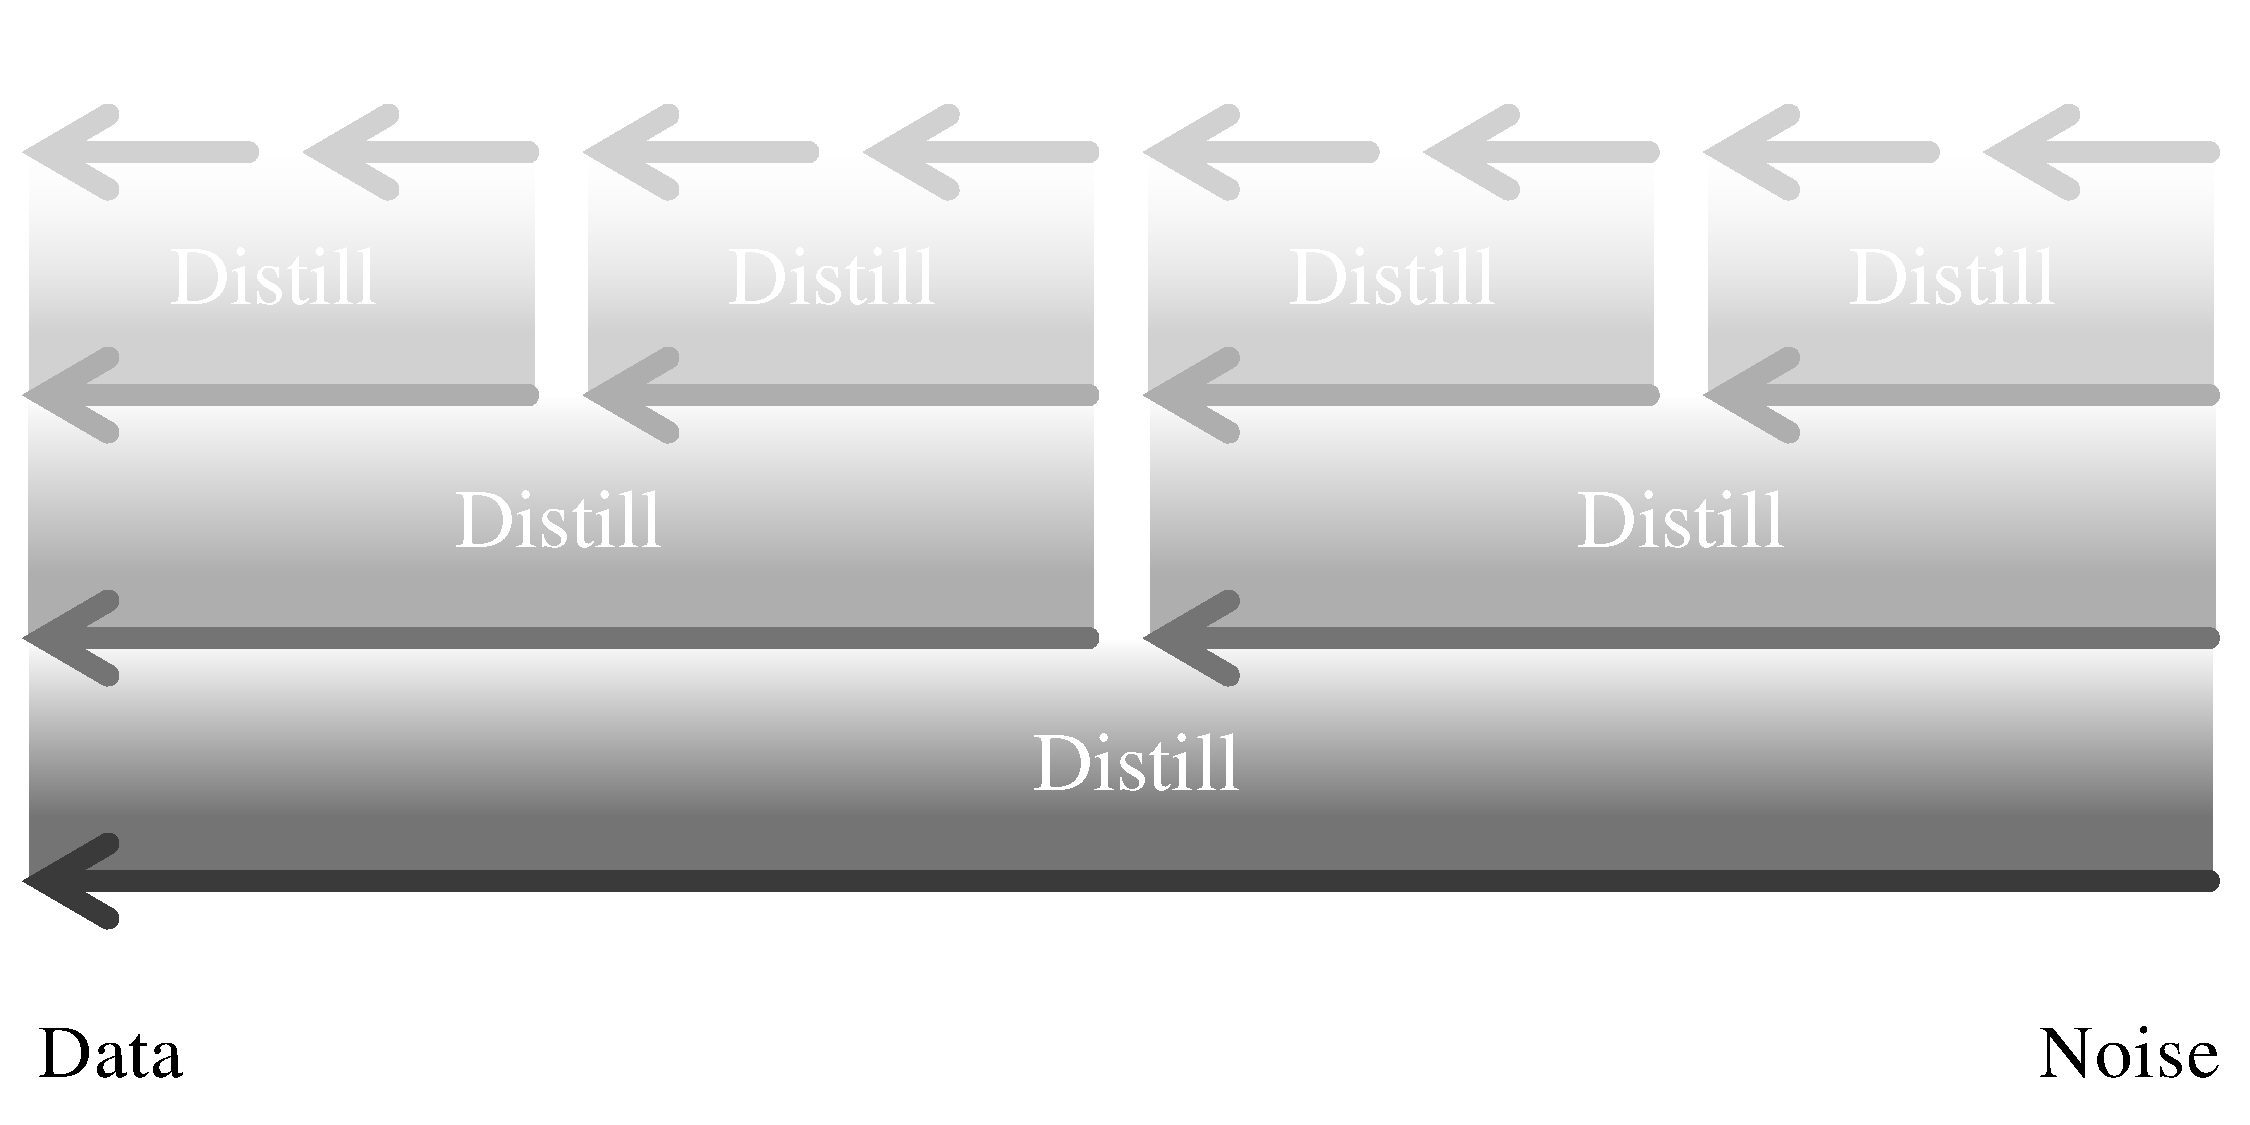
\includegraphics[width=0.93\linewidth]{Images/PartD/PD.pdf} 
    \caption{\textbfs{渐进蒸馏（PD）示意。}
每一轮训练学生时，都要求学生的单步复现教师相邻两步的效果。
这一过程把教师的 $N$ 个区间蒸馏成 $N/2$ 个学生步，再反复进行，
逐步把轨迹长度减半，直到达到所需的步数。箭头表示多步的教师转移
如何被压缩为更少的学生步，从噪声走向数据。
\figcredit{由作者绘制。}
}
    \label{fig:pd-illustration}
\end{figure}



下面先介绍 PD 的蒸馏操作 \Cref{subsec:pd-distillation}，
再总结整个训练流程 \Cref{subsec:pd-training}，
\Cref{subsec:pd-guidance} 则给出对 CFG 引导的扩展。


\subsection{PD 中的蒸馏操作}\label{subsec:pd-distillation}

本节把采用 $\rvx$-预测参数化的 DDIM 作为时间步进规则，
并仍用 $\mathtt{Solver}_{s \to t}$ 表示代入当前教师的
$\rvx$-DDIM 去噪器后所得的确定性映射。在 PD 的第一轮中
（教师就是预训练的扩散模型），这与用 DDIM 积分扩散 PF-ODE 是一致的；
而在后面几轮中（教师换成以前的学生），$\mathtt{Solver}_{s \to t}$
只是当前教师所诱导的 DDIM 转移，而不再是原始的扩散 PF-ODE。
蒸馏步骤如下：从噪声输入 $\rvx_s$ 出发（即干净数据的一个受扰版本，
$\rvx_s = \alpha_s \rvx_0 + \sigma_s \bm{\epsilon}$），训练学生去预测
目标 ${\color{orange}\tilde\rvx}$，使得学生走一步 $s\!\to\! t$ 就能
复现教师连续两步 $s\!\to\! u\!\to\! t$ 的结果。记
$\rvx_{\bm{\phi}^\times}(\rvx,\tau)$ 为教师在本轮的 $\rvx$-预测去噪器。
连续施加两次教师诱导的 DDIM 转移，得到
\[
\tilde\rvx_u := \mathtt{Solver}_{s\to u}\!\left(\rvx_s;\,\rvx_{\bm{\phi}^\times}\right),
\qquad
\tilde\rvx_t := \mathtt{Solver}_{u\to t}\!\left(\tilde\rvx_u;\,\rvx_{\bm{\phi}^\times}\right).
\]
这里的记号沿用 \Cref{eq:solver}，表示以 $\rvx_s$ 为起点、从 $s$ 到 $t$
的确定性转移映射，其中 $\rvx_{\bm{\phi}^\times}$ 按 DDIM 的方式代入。

\begin{question}
在时刻 $s$ 应当取什么「伪干净」目标 ${\color{orange}\tilde\rvx}$，
才能使求解器直接从 $s \to t$ 一步走出的结果 $\tilde\rvx_t$
与经 $s \to u \to t$ 两步走出的结果相同？
具体地说，求满足下式的 ${\color{orange}\tilde\rvx}$：
\[
\tilde\rvx_t = \mathtt{Solver}_{s\to t}\left(\rvx_s; {\color{orange}\tilde\rvx}\right).
\]
\end{question}





一旦得到 ${\color{orange}\tilde\rvx}$ 的闭式表达，就训练一个学生模型
$\rvf_{\bm{\theta}}(\rvx_s, s)$（这里同样是 $\rvx$-预测模型），
让它逼近这个「两步合一」目标 ${\color{orange}\tilde\rvx}$，
即最小化
\begin{align}\label{eq:pd-optimization}
\min_{\bm{\theta}} \E_s
\mathbb{E}_{\rvx_s\sim p_s}\!\left[w(\lambda_s)\,\big\|\rvf_{\bm{\theta}}(\rvx_s, s) - {\color{orange}\tilde\rvx}\big\|_2^2\right].
\end{align}


下面说明：在 DDIM 规则下，${\color{orange}\tilde\rvx}$ 有初等代数形式的
闭式表达（该结果对离散时间与连续时间都成立）：
\lemp{DDIM 下的两步合一目标 ${\color{orange}\tilde\rvx}$}{pd-ddim}{以 $\rvx_s$ 为初始条件，若求解器采用 DDIM，则「两步合一」目标 ${\color{orange}\tilde\rvx}$ 可按下式计算
\begin{align*}
    {\color{orange}\tilde\rvx} 
    &=\frac{\sigma_s}{\alpha_t\sigma_s - \alpha_s\sigma_t} \tilde\rvx_t - \frac{\sigma_t}{\alpha_t\sigma_s - \alpha_s\sigma_t} \rvx_s.
\end{align*}
其中 $\tilde\rvx_t$ 是沿 $s \to u \to t$ 把 DDIM（\Cref{eq:ddim-update-all}）施加两次得到的：
\begin{align*}
    s \to u: & \quad    && \tilde\rvx_u = \frac{\sigma_u}{\sigma_s}\rvx_s + \alpha_s \left(\frac{\alpha_u}{\alpha_s} - \frac{\sigma_u}{\sigma_s} \right)\rvx_{\bm{\phi}^\times}(\rvx_s, s)  \\
    u \to t: & \quad    && \tilde\rvx_t = \frac{\sigma_t}{\sigma_u}\tilde\rvx_u + \alpha_u \left(\frac{\alpha_t}{\alpha_u} - \frac{\sigma_t}{\sigma_u} \right)\rvx_{\bm{\phi}^\times}(\tilde\rvx_u, u).
\end{align*}
}{$\tilde\rvx_t$ 必须等于从 $s$ 到 $t$ 一步 DDIM 的结果
$\tilde\rvx_t'$，而后者写作：
\[
s \to t: \quad \tilde\rvx_t' = \frac{\sigma_t}{\sigma_s}\rvx_s + \alpha_s \left(\frac{\alpha_t}{\alpha_s} - \frac{\sigma_t}{\sigma_s} \right) {\color{orange}\tilde\rvx}.
\]
令 $\tilde\rvx_t'$ 与 $\tilde\rvx_t$ 相等，即可解出
${\color{orange}\tilde\rvx}$ 关于 $\tilde\rvx_t$、$s$ 与 $t$ 的表达式：
\begin{align}
    &\tilde\rvx_t = \tilde\rvx_t' \nonumber \\
    \Longleftrightarrow\,\, & \tilde\rvx_t = \frac{\sigma_t}{\sigma_s}\rvx_s + \alpha_s \left(\frac{\alpha_t}{\alpha_s} - \frac{\sigma_t}{\sigma_s} \right) {\color{orange}\tilde\rvx} \nonumber \\
    \Longleftrightarrow\,\, & {\color{orange}\tilde\rvx} =  \frac{\tilde\rvx_t - \frac{\sigma_t}{\sigma_s}\rvx_s}{\alpha_s \left(\frac{\alpha_t}{\alpha_s} - \frac{\sigma_t}{\sigma_s} \right)} \label{eq:x-pd-paper} \\
    \Longleftrightarrow\,\, & {\color{orange}\tilde\rvx} = \frac{\sigma_s}{\alpha_t\sigma_s - \alpha_s\sigma_t} \tilde\rvx_t - \frac{\sigma_t}{\alpha_t\sigma_s - \alpha_s\sigma_t} \rvx_s. \nonumber
\end{align}
}
借助这一公式，PD 便算出了时刻 $s$ 的伪干净目标：
学生的单个 DDIM 步 $s\!\to\!t$ 正好落在两步结果 $\tilde\rvx_t$ 处。


\paragraph{实用的离散时间网格与损失。}
实际使用时，先固定一个递减的网格 $t_0=T>t_1>\cdots>t_N=0$，
为书写简洁再记 $s:=t_k$、$u:=t_{k+1}$、$t:=t_{k+2}$。
教师提供各一步映射 $\mathtt{Teacher}_{t_k\to t_{k+1}}$，
而学生要学的则是与教师映射复合相匹配的两步跳跃映射：
\[
\mathtt{Student}_{t_k\to t_{k+2}}
 \approx 
\mathtt{Teacher}_{t_{k+1}\to t_{k+2}}
\circ
\mathtt{Teacher}_{t_{k}\to t_{k+1}}.
\]

对标准的减半调度，设 $N$ 为偶数，并抽取时间三元组
$(s,u,t)=(t_k,t_{k+1},t_{k+2})$，其中
$k\in\{0,2,\ldots,N-2\}$。此时目标 \Cref{eq:pd-optimization} 变为
\[
\min_{\bm{\theta}} 
\mathbb{E}_{\,k \sim \mathcal{U}\{0,2,\ldots,N{-}2\}}
\mathbb{E}_{\,\rvx_{t_k}\sim p_{t_k}}\!
\Big[
  w(\lambda_{t_k})\,
  \big\|
  \rvf_{\bm{\theta}}(\rvx_{t_k},t_k) - {\color{orange}\tilde\rvx}^{(k)}
  \big\|_2^2
\Big],
\]
其中教师给出的两步目标 ${\color{orange}\tilde\rvx}^{(k)}$ 由引理
~\ref{pd-ddim} 算出。若网格是均匀的，可写成 $t_k = T(1 - k/N)$，于是
\[
s = T\Big(1 - \frac{k}{N}\Big),\quad
u = T\Big(1 - \frac{k+1}{N}\Big),\quad
t = T\Big(1 - \frac{k+2}{N}\Big),
\]
对应着间距均匀的时间步长 $\Delta s = T/N$。


\subsection{PD的整个训练流程及其采样}\label{subsec:pd-training}
在这些局部配对片段上按 \Cref{eq:pd-optimization} 训练完毕之后，
$\mathtt{Student}$ 就不再走原网格的每一个区间：它的每一步都覆盖
$\mathtt{Teacher}$ 连续的两步，因此每隔一个时间点前进一步，
\[
t_0 \to t_2 \to t_4 \to \cdots \to t_N,
\]
于是跨越同样的时间范围 $[0,T]$ 只需 $N/2$ 次转移。这一阶段结束后，
训练好的 $\mathtt{Student}$ 取代 $\mathtt{Teacher}$ 成为新的去噪器。
随后在更粗的网格上（时间步长加倍）重复整个过程，得到序列
\[
N \;\to\; N/2 \;\to\; N/4 \;\to\; \cdots,
\]
直到达到所需的推理步数。每一轮迭代中，新的 $\mathtt{Student}$
都从更新后的 $\mathtt{Teacher}$ 初始化而来。这种反复对半的做法
在保留全局时间范围的同时，逐步压缩生成过程的时间分辨率。

\paragraph{采样。}
推理时用（DDIM）求解器配合当前的 $\mathtt{Student}$ 作为去噪器，
采样器在训练所得的那套更粗的网格上前进。第一轮结束后走的是
「跳 2 步」（$t_0 \to t_2 \to \cdots \to t_N$），下一轮之后改成
「跳 4 步」（$t_0 \to t_4 \to \cdots \to t_N$），依此类推。
每一轮迭代都把采样步数减半，而起点与终点时间保持不变。

\subsection{补充讨论：局部半群匹配与更一般的求解器}


\paragraph{渐进蒸馏作为局部半群匹配。}
在统一目标 \Cref{eq:general-cm-loss} 中，难以直接计算的预言量目标
$\bPsi_{s\to 0}$ 被一个由教师诱导的替身取代，所用的是 ODE 流的
\emph{半群性质}（详见后文 \Cref{eq:semi-group}）：从 $s$ 演化到 $t$，
应当等价于先从 $s$ 走到任一中间时刻 $u$、再从 $u$ 走到 $t$，即
\[
\bPsi_{s\to t} = \bPsi_{u\to t}\circ\bPsi_{s\to u}.
\]
PD 是在局部施加这一要求：训练学生的单步映射去匹配教师两个相邻
单步片段的复合，即
\begin{align}\label{eq:pd-local}
  \E_{s}\E_{\rvx_s\sim p_s}
  \big\|
    \underbrace{\rmG_{\btheta}(\rvx_s, s, s-2\Delta s)}_{\text{学生的单步}}
    -
    \underbrace{\mathtt{Solver}_{s-\Delta s\to s-2\Delta s}\big(\mathtt{Solver}_{s\to s-\Delta s}(\rvx_s)\big)}_{\text{教师两步的复合}}
  \big\|_2^2.
\end{align}
当教师所用的求解器能准确逼近底层的 ODE 流时，
\Cref{eq:pd-local} 就在很短的递减网格上近似了相应的半群关系
（取 $s>u>t$，其中 $u=s-\Delta s$、$t=s-2\Delta s$）：
\begin{align*}
  \bPsi_{s\to s-2\Delta s}
  &= \bPsi_{s-\Delta s\to s-2\Delta s}\circ\bPsi_{s\to s-\Delta s}
  \\&\approx
  \mathtt{Solver}_{s-\Delta s\to s-2\Delta s}\circ \mathtt{Solver}_{s\to s-\Delta s},
\end{align*}
因此训练只需要教师的一小段局部片段，而不必把轨迹从 $s$ 一直展开到 $0$。
为回到 \Cref{eq:general-cm-loss} 中少步去噪器的视角，
把学生的少步映射定义为各个已学跳跃映射的复合：
\[
\underbrace{\rmG_{\btheta}(\rvx_s, s, 0)}_{\text{少步去噪器}}
=
\big(\rmG_{\btheta}(\,\cdot\,, 2\Delta s, 0)\circ\cdots\circ \rmG_{\btheta}(\,\cdot\,, s, s-2\Delta s)\big)(\rvx_s).
\]
从概念上说，\Cref{eq:pd-local} 为下面的全局回归提供了一个高效的
\emph{局部替身}：
\[
\E_{s,\rvx_s}\Big\|\rmG_{\btheta}(\rvx_s,s,0)\;-\;(\mathtt{Solver})^{\circ}_{s\to 0}(\rvx_s)\Big\|_2^2,
\]
其中 $(\mathtt{Solver})^{\circ}_{s\to 0}$ 表示在步长为 $\Delta s$ 的网格上，
教师映射从 $s$ 到 $0$ 的完整复合，用来充当 $\bPsi_{s\to 0}$ 的替身。

\paragraph{能否改用别的求解器？}
上面的推导中，我们在 $\rvx$-预测参数化下用 DDIM 作为具体的
PF-ODE 采样器。但基本的蒸馏原理更为一般：只要教师的若干步
能给出目标终点，再训练学生用更粗的一步到达同一个终点即可。

只要较粗那一层的求解器更新可以依据学生的网络预测反解出来，
前面导出的闭式伪目标就同样可用。
对 DDIM 来说，更新式关于单个 $\rvx$ 预测是仿射的，
所以这一反解可以解析地完成。同样的思路也适用于其他
一步更新允许类似反解的求解器。

而对更复杂的求解器，这种「由单个输出反解」的做法未必可行：
多阶段方法要用多次网络评估，多步方法依赖先前的求解器状态，
隐式方法还要解耦合方程。此时可以改为直接算出较粗的学生步，
再把它与教师细步所得的端点按 \Cref{eq:pd-local} 直接匹配，
并在可行时让梯度穿过求解器回传给学生。另外要注意，
较粗的步本身可能就要用多次网络评估，因此时间步数变少
并不一定意味着 NFE 同比例减少。

对随机采样器而言，同样的路径匹配逻辑要成立，
就必须让教师与学生固定或耦合使用同一组随机抽样。
若没有这种耦合，各条轨迹就不必共享同一个端点，
此时合适的目标通常是分布匹配，而非路径匹配。


































































































































\subsection{带引导的渐进蒸馏}\label{subsec:pd-guidance}
\citet{meng2023distillation} 给出了一个两级流程，用于蒸馏
带无分类器引导（CFG）的扩散模型：（1）把引导「提取」进一个
以引导强度为输入的单网络中；（2）再用\emph{渐进式蒸馏（PD）}
减少采样步数。他们在像素空间与隐空间（例如 Stable Diffusion）
上都验证了这一做法。

\paragraph{第一级蒸馏：把引导蒸馏掉。}
记 $\rvx_{\bm{\phi}^\times}(\rvx_s, s, \rvc)$ 为（预训练的）条件扩散模型
在「$\rvx$-预测」参数化下的输出（即干净数据估计），时刻为 $s$、
条件为 $\rvc$；条件也可以取空，即 $\rvc=\emptyset$（无条件分支）。
\Cref{eq:cfg-model-nn} 中带权 $\omega$ 的 CFG 组合可以写成
\begin{equation}\label{eq:cfg-model-clean}
   \rvx_{\bm{\phi}^\times}^{\,\omega}(\rvx_s, s, \rvc)
   := (1+\omega)\,\rvx_{\bm{\phi}^\times}(\rvx_s, s, \rvc)
      - \omega\,\rvx_{\bm{\phi}^\times}(\rvx_s, s, \emptyset),
\end{equation}
其中 $\omega \sim p_\omega(\omega)$ 取自某个 CFG 权重分布 $p_\omega$，
通常取 $p_\omega(\omega)=\mathcal{U}[\omega_{\min},\omega_{\max}]$。
第一级引入一个新模型 $\rvx_{\bm{\theta}_1}(\rvx_s, s, \rvc, \omega)$，
它直接把 $\omega$ 作为输入，通过回归去复现 CFG 的监督输出
$\rvx_{\bm{\phi}^\times}^{\,\omega}(\rvx_s, s, \rvc)$：
\[
\min_{\bm{\theta}_1}\;
\mathbb{E}_{\omega\sim p_\omega, s, \rvx\sim p_{\mathrm{data}}, \rvx_s \sim p(\rvx_s\mid \rvx)}
\lambda(s)
\big\|\rvx_{\bm{\theta}_1}(\rvx_s, s, \rvc, \omega)-\rvx_{\bm{\phi}^\times}^{\omega}(\rvx_s, s, \rvc)\big\|_2^2.
\]
这里 $\lambda(s)$ 是与调度相关的标准权重；每次迭代都重新抽取
$\omega$，从而使单个网络学会模拟任意强度的 CFG 引导。

\paragraph{第二级蒸馏：PD。}
第一级得到的模型 $\rvx_{\bm{\theta}_1}(\rvx_s, s, \rvc, \omega)$
在 PD 中充当教师，按 \Cref{subsec:pd-training} 的方式逐步蒸馏成
采样步数更少的学生 $\rvx_{\bm{\theta}_2}(\rvx_s, s, \rvc, \omega)$。
每轮迭代都把步数减半（例如 $N \to N/2 \to N/4 \to \cdots$）。

\newpage
\section{结束语}\label{sec:ch10_cr}

本章介绍了我们遇到的第一个基于训练的加速范式。在把无需训练的改进
通过数值求解器用尽之后，我们把关注点转向一条新策略：训练一个快速的
\textit{学生}生成器，让它学会复制那个缓慢的、预训练的\textit{教师}
扩散模型的行为。

我们考察了两条主要的蒸馏原理。其一是分布层面的蒸馏，以变分分数蒸馏
（VSD）等方法为代表：训练学生的输出分布去对齐教师的输出分布，
做法是在各个噪声水平上调准二者的分数函数，从而给出稳定、
非对抗式的目标。其二是流映射层面的蒸馏，我们看到渐进蒸馏（PD）
这类方法如何训练学生直接逼近教师的解轨迹；PD 的迭代做法
（每轮把采样步数减半）被证明是把漫长的迭代过程压缩到几步的
有力且实用的手段。

这些蒸馏技术成功弥补了迭代式扩散模型的高样本质量与一步生成器的
推理速度之间的落差，为高效、高保真的合成提供了一条很有吸引力的路径。

然而，依赖预训练教师也带来了两段式的流程：先训练一个缓慢但强大的教师，
再把它蒸馏成快速的学生。这就在生成模型研究的前沿引出一个基本问题：
能否完全绕开教师？

是否可以设计一套独立的训练原理，直接从数据中学出这些快速、少步的生成器？
本书的最后一章将回答这个问题。
\begin{enumerate}
    \item 我们将考察一致性模型这类开创性方法，它们能学出从 ODE 轨迹上任意一点到其终点的映射。
    \item 我们还将深入讨论一致性模型的推广形式，即学会把 ODE 轨迹上的任意一点一步映射到轨迹上的另一点。
\end{enumerate}
从改进求解器、从教师那里「提取」解，转而直接学习解映射本身，
这一转变代表了迈向一类新型生成模型的重要一步——这类模型在设计上
既有原则性，又足够高效。

\clearpage
\newpage